\PassOptionsToPackage{unicode=true}{hyperref} % options for packages loaded elsewhere
\PassOptionsToPackage{hyphens}{url}
%
\documentclass[]{article}
\usepackage{lmodern}
\usepackage{amssymb,amsmath}
\usepackage{ifxetex,ifluatex}
\usepackage{fixltx2e} % provides \textsubscript
\ifnum 0\ifxetex 1\fi\ifluatex 1\fi=0 % if pdftex
  \usepackage[T1]{fontenc}
  \usepackage[utf8]{inputenc}
  \usepackage{textcomp} % provides euro and other symbols
\else % if luatex or xelatex
  \usepackage{unicode-math}
  \defaultfontfeatures{Ligatures=TeX,Scale=MatchLowercase}
\fi
% use upquote if available, for straight quotes in verbatim environments
\IfFileExists{upquote.sty}{\usepackage{upquote}}{}
% use microtype if available
\IfFileExists{microtype.sty}{%
\usepackage[]{microtype}
\UseMicrotypeSet[protrusion]{basicmath} % disable protrusion for tt fonts
}{}
\IfFileExists{parskip.sty}{%
\usepackage{parskip}
}{% else
\setlength{\parindent}{0pt}
\setlength{\parskip}{6pt plus 2pt minus 1pt}
}
\usepackage{hyperref}
\hypersetup{
            pdftitle={The 2019-20 NBA Season: What Could Have Been},
            pdfauthor={Ryan Kohanski; Rithvik Saravanan; Howard Yong},
            pdfborder={0 0 0},
            breaklinks=true}
\urlstyle{same}  % don't use monospace font for urls
\usepackage[margin=1in]{geometry}
\usepackage{graphicx,grffile}
\makeatletter
\def\maxwidth{\ifdim\Gin@nat@width>\linewidth\linewidth\else\Gin@nat@width\fi}
\def\maxheight{\ifdim\Gin@nat@height>\textheight\textheight\else\Gin@nat@height\fi}
\makeatother
% Scale images if necessary, so that they will not overflow the page
% margins by default, and it is still possible to overwrite the defaults
% using explicit options in \includegraphics[width, height, ...]{}
\setkeys{Gin}{width=\maxwidth,height=\maxheight,keepaspectratio}
\setlength{\emergencystretch}{3em}  % prevent overfull lines
\providecommand{\tightlist}{%
  \setlength{\itemsep}{0pt}\setlength{\parskip}{0pt}}
\setcounter{secnumdepth}{0}
% Redefines (sub)paragraphs to behave more like sections
\ifx\paragraph\undefined\else
\let\oldparagraph\paragraph
\renewcommand{\paragraph}[1]{\oldparagraph{#1}\mbox{}}
\fi
\ifx\subparagraph\undefined\else
\let\oldsubparagraph\subparagraph
\renewcommand{\subparagraph}[1]{\oldsubparagraph{#1}\mbox{}}
\fi

% set default figure placement to htbp
\makeatletter
\def\fps@figure{htbp}
\makeatother


\title{The 2019-20 NBA Season: What Could Have Been}
\author{Ryan Kohanski \and Rithvik Saravanan \and Howard Yong}
\date{May 11, 2020}

\begin{document}
\maketitle

\hypertarget{introduction}{%
\subsection{Introduction}\label{introduction}}

Due to the widespread impact of COVID-19 throughout the world, almost
every company, organization, and public event has canceled or suspended
any activities that involve interpersonal contact for the forseeable
future. Many of these activities are moving to a virtual format if
possible, but several others have been forced to shut down.

As avid sports fans, the absence of the major sporting events during
this time has hit us and many others around the world especially hard. A
full list of all sporting events canceled around the world during the
coronavirus can be found
\href{https://www.espn.com/olympics/story/_/id/28824781/list-sporting-events-canceled-coronavirus}{here}.
Some of the events that we particularly were looking forward to include
the NBA, NCAA March Madness tournament, MLB, and the 2020 Summer
Olympics.

In our curiosity, we decided to utilize this opportunity to exercise our
data science and modeling skills in order to predict what could have
been. Specifically, we focused on the NBA and the NBA Playoffs. Since
the 2019-20 NBA season was suspended approximately one month prior to
the end of the regular season (and the beginning of the playoffs), we
used the 2019-20 season data accumulated from the games played before
the suspension to predict how the season and the playoffs would have
ended had everything gone according to schedule.

In this analysis, we will examine data from the 2019-20 NBA season as
well as some data from previous NBA seasons in order to draw some
meaningful conclusions about the remainder of the 2019-20 NBA season.

\hypertarget{predicting-the-2019-20-nba-season}{%
\subsection{Predicting the 2019-20 NBA
Season}\label{predicting-the-2019-20-nba-season}}

Since we missed one of the most exciting times of the year (the NBA
Playoffs \& Finals), we made some predictions on how the rest of the
season might have played out using a popular methodology referred to as
the \href{https://en.wikipedia.org/wiki/Elo_rating_system}{Elo ratings
system}. This tool, created by Hungarian-American physics professor
Arpad Elo, was orginally designed to rate chess players, but is now used
for all sorts of competitions ranging anywhere from sports to video
games. This is a methodology that
\href{https://fivethirtyeight.com/features/how-we-calculate-nba-elo-ratings/}{FiveThirtyEight}
and many other popular sports analysts take advantage of due to its
simplicity and effectiveness.

These ratings depend only on the final score of each game as well as
where it was played (home-court advantage). In other words, this system
is built on a Win/Loss basis. We will be analyzing the 2018-19 NBA
Season in its entirety to validate its performance, then we will apply
it to the 2019-20 regular season in order to predict the matchups for
the Playoffs and the Finals and ultimately the NBA Champions. For this
project, we retrieved several types of data sources including
game-by-game scores and schedules for several seasons from
\href{https://www.basketball-reference.com/}{Basketball-Reference.com}.

\hypertarget{how-does-elo-work}{%
\paragraph{How does Elo work?}\label{how-does-elo-work}}

The long-run average for an Elo score in the NBA sits around 1500. An
Elo of 1500 means that the teams performance would be normally
distrubuted around an average of 1500 with the chance of performing
better or worse. The formula for Elo below shows how the probability of
one team beating another is calculated using the ratings.

When Player \(A\) competes in a match against Player \(B\), Player \(A\)
has an expected outcome (probability or score) for Team \(A\) (\(E[A]\))
where \(R_A\) is the rating for Team \(A\) and \(R_B\) is the rating for
Team \(B\). The expected outcome for Team \(A\) (\(E[A]\)) can be
calculated by the formula below:

\[
\begin{aligned}
  \textrm{E[A]} & = \frac{1}{1 + 10^{\frac{(R_B-R_A)}{400}}}
\end{aligned}
\]

The same calculation (\(E[B]\)) has to be done for Player \(B\), but
with \(R_A\) (current rating \(A\)) and \(R_B\) (current rating \(B\))
swapped so that \(E[A] + E[B] = 1\). Once the match is played and
\(S_A\) (actual outcome or score for Team \(A\)), and \(S_B\) (actual
outcome or score for Team \(B\)) are determined, \(R^{\prime}_A\) (New
rating for \(A\)) and \(R^{\prime}_B\) (New rating for \(A\)) are
calculated with the formula below:

\[
\begin{aligned}
  R^{\prime}_A=R_A+K(S_A−E[A])
\end{aligned}
\]

The \(S\) value in our case would either be 1 for a win, or 0 for a
loss. This is because there are no ties in the NBA.

In this equation, \(K\) is an optimization constant that usually takes
different values according the sport and the amount of games available.
In other words, this value is the maximum amount by which a score can
change in one match. If \(K\) is set too high, the ratings will jump
around too much; if \(K\) is set too low, Elo will take too long to
recognize important changes in team quality. Determining the right value
of K is an entirely different and more complicated topic, so for this
experiment we will be using \(K=20\), the optimal \(K\) for the NBA
determined by
\href{https://fivethirtyeight.com/features/how-we-calculate-nba-elo-ratings/}{FiveThirtyEight}.
This is higher than most other sports and can likely be attributed to
the fact that the NBA plays more games (81 games per team) and is
subject to relatively little randomness.

Home-court advantage is set as equivalent to 100 Elo rating points. One
hundred Elo points is equivalent to about 3.5 NBA points, so it can also
be interpreted as the home team being favored by 3 to 4 points if the
teams were otherwise evenly matched (obviously this value fluctuates
from season to season). Since every team plays about half of their games
at home and the other half away, a change in the home-court advantage
value does not produce a significant difference in the ratings, but is
still an important factor to consider.

Elo strikes a nice balance between ratings systems that account for
margin of victory and those that do not. While teams always gain Elo
points after wins and lose Elo points after losses, they also gain or
lose more with larger margins of victory.

This works by assigning a multiplier to each game based on the final
score and dividing it by a team's projected margin of victory
conditional upon having won the game. For instance, the Golden State
Warriors' 4-point margin over the Houston Rockets in Game 1 of the
2018-19 Western Conference finals was lower than Elo would expect for a
Warriors win. So the Warriors gain Elo points, but not as many as if
they'd won by a larger margin. The formula accounts for diminishing
returns; going from a 5-point win to a 10-point win matters more than
going from a 25-point win to a 30-point win. For the exact formula, see
the footnotes.

Instead of resetting each team's rating when a new season begins, Elo
carries over a portion of a team's rating from one season to the next.
This is to account for any momentum that a team may build from
season-to-season (i.e.~sports dynasties). In NBA ratings, three-quarters
of the previous score are kept. The high fraction reflects the fact that
NBA teams are more consistent from year to year. For example, the Miami
Heat ended the 2012-13 NBA season with an Elo rating of 1754. The team's
Elo rating for the start of the 2013-14 season is calculated as follows:

\[
\begin{aligned}
  (0.75 * 1754) + (0.25 * 1500) = 1692
\end{aligned}
\]

Since this is a consistent method, we will also initialize the Elo
scores for the 2019-20 NBA Season using the Elo scores from the 2018-19
season.

After incorporating a constant for home court advantage, our formula is
as follows with \(A=100\) points (the value we previously determined
represetns a home-court advantage):

\[
\begin{aligned}
  P(\textrm{Home team wins}) & = \frac{1}{1 + 10^{-\frac{(H-R+A)}{400}}}
\end{aligned}
\]

This is an example of a logistic function:

\begin{center}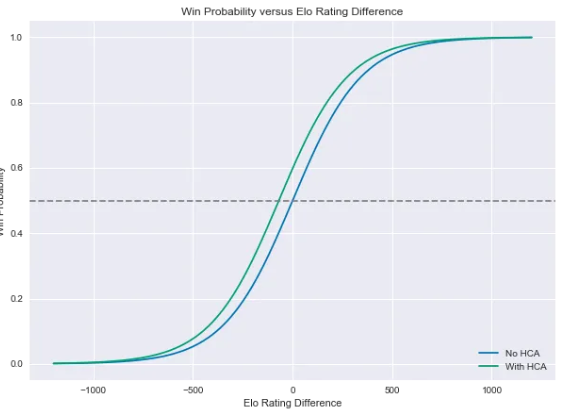
\includegraphics[width=.49\linewidth]{./logistic2} \end{center}

\hypertarget{the-2018-19-nba-season}{%
\paragraph{The 2018-19 NBA Season}\label{the-2018-19-nba-season}}

\end{document}
